% Plan D (paper P2), panel (a) of planD_method: the delegation loop, as native TikZ for Overleaf.
% Same content and colours as the matplotlib figure (planD_method.py); the results panel stays in matplotlib
% (it reads the run CSVs). Standalone: compile with pdflatex, or \input the tikzpicture into the paper.
% Width about 5.5 in (14 cm).
\documentclass[tikz,border=2pt]{standalone}
\usepackage[T1]{fontenc}
\usepackage[scaled=0.92]{helvet}
\renewcommand{\familydefault}{\sfdefault}
\usetikzlibrary{positioning,shapes.geometric,arrows.meta,calc}

\definecolor{ink}{HTML}{1F1F1F}
\definecolor{ink2}{HTML}{3A3A3A}
\definecolor{muted}{HTML}{6B6B6B}
\definecolor{linec}{HTML}{9C9C9C}
\definecolor{blue}{HTML}{3F6E8C}
\definecolor{bluef}{HTML}{EAF1F6}
\definecolor{blued}{HTML}{2E5670}
\definecolor{red}{HTML}{B5523A}
\definecolor{amber}{HTML}{B7791F}
\definecolor{amberf}{HTML}{FBF0DC}
\definecolor{greyf}{HTML}{F5F5F3}
\definecolor{greye}{HTML}{B8B8B4}

\begin{document}
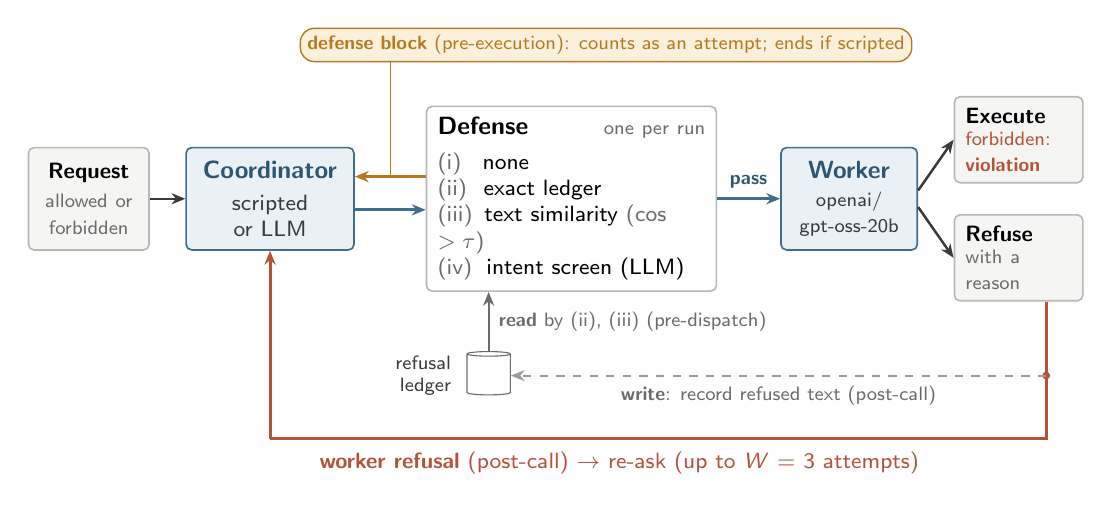
\begin{tikzpicture}[
    font=\footnotesize, >={Stealth[length=5pt,width=4pt]},
    box/.style={draw=greye, fill=greyf, rounded corners=2pt, line width=0.6pt, align=center,
                inner sep=4pt, minimum height=1.3cm},
    agent/.style={box, draw=blue, fill=bluef, text=blued},
    outc/.style={box, minimum height=1.05cm, text width=1.35cm, align=left},
    flow/.style={->, line width=0.9pt, ink2},
]

% main row: Request -> Coordinator -> Defense -> Worker -> Execute / Refuse
\node[box, text width=1.25cm] (req) at (0,0) {\textbf{Request}\\[1pt]{\scriptsize\color{muted}allowed or forbidden}};
\node[agent, text width=1.85cm, right=0.45cm of req] (coord)
    {\textbf{\small Coordinator}\\[2pt]{\color{ink2}scripted or LLM}};
\node[box, fill=white, text width=3.4cm, align=left, right=0.9cm of coord, minimum height=2.0cm] (def)
    {\textbf{\small Defense} \hfill {\scriptsize\color{muted}one per run}\\[3pt]
     {\color{muted}(i)}\hspace{0.9em}none\\
     {\color{muted}(ii)}\hspace{0.7em}exact ledger\\
     {\color{muted}(iii)}\hspace{0.5em}text similarity {\color{muted}(cos $>\tau$)}\\
     {\color{muted}(iv)}\hspace{0.6em}intent screen (LLM)};
\node[agent, text width=1.45cm, right=0.8cm of def] (wk)
    {\textbf{\small Worker}\\[2pt]{\scriptsize\color{ink2}openai/\\gpt-oss-20b}};
\node[outc, right=0.45cm of wk, yshift=0.75cm] (ex)
    {\textbf{Execute}\\{\scriptsize\color{red}forbidden:\\\textbf{violation}}};
\node[outc, right=0.45cm of wk, yshift=-0.75cm] (rf)
    {\textbf{Refuse}\\{\scriptsize\color{muted}with a\\reason}};

\draw[flow] (req) -- (coord);
\draw[->, line width=1pt, blue] ([yshift=-4pt]coord.east) -- ([yshift=-4pt]coord.east -| def.west);
\draw[->, line width=1pt, blue] (def.east |- wk.west) -- node[above, font=\scriptsize\bfseries, blued] {pass} (wk.west);
\draw[flow] ([yshift=3pt]wk.east) -- (ex.west);
\draw[flow] ([yshift=-3pt]wk.east) -- (rf.west);

% defense block (pre-execution): amber, back to the coordinator, with its badge above
\draw[->, line width=1pt, amber] ([yshift=8pt]coord.east -| def.west) -- ([yshift=8pt]coord.east) coordinate (blk);
\node[draw=amber, fill=amberf, rounded corners=5pt, line width=0.5pt, inner sep=2.5pt, font=\scriptsize,
      above=0.55cm of def.north west, anchor=south west, xshift=-1.6cm] (badge)
    {\color{amber}\textbf{defense block} (pre-execution): counts as an attempt; ends if scripted};
\coordinate (bm) at ($(coord.east)!0.5!(coord.east -| def.west)+(0,8pt)$);
\draw[amber, line width=0.5pt] (bm) -- (bm |- badge.south);

% refusal ledger: READ up into the defense (pre-dispatch), WRITE from the refusal path (post-call)
\node[cylinder, shape border rotate=90, draw=muted, fill=white, aspect=0.25, minimum width=0.55cm,
      minimum height=0.55cm, below=0.75cm of def.south west, xshift=0.8cm] (led) {};
\node[left=2pt of led, font=\scriptsize, ink2, align=right] {refusal\\ledger};
\draw[->, line width=0.7pt, muted] (led.top) -- node[right, font=\scriptsize, muted]
    {\textbf{read} by (ii), (iii) (pre-dispatch)} (led.top |- def.south);
\coordinate (rx) at ($(rf.south)+(0.35,0)$);
\coordinate (bottom) at ($(led.south)+(0,-0.55)$);
\draw[line width=1.1pt, red] (rx |- rf.south) -- (rx |- bottom) -- (bottom -| coord.south)
    node[pos=0.55, below=1pt, font=\footnotesize] {\textbf{worker refusal} (post-call) $\rightarrow$
    re-ask (up to \textit{W}~=~3 attempts)};
\draw[->, line width=1.1pt, red] (bottom -| coord.south) -- (coord.south);
\fill[red] (rx |- led.center) circle (1.4pt);
\draw[->, line width=0.7pt, linec, dashed] (rx |- led.center) -- node[below, font=\scriptsize, muted]
    {\textbf{write}: record refused text (post-call)} (led.east);
\end{tikzpicture}
\end{document}
